\documentclass[tikz]{standalone}
\usepackage{bm}
\usepackage{stix}

\usetikzlibrary{calc}

\definecolor{mplblue}{HTML}{1f77b4}

\tikzstyle{site}=[rounded corners, minimum size=0.7cm, draw=mplblue!80!black, fill=mplblue!20!white]

\begin{document}
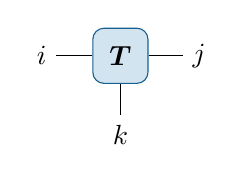
\begin{tikzpicture}[x=2cm, y=2cm]

\node [site] (T) at (0, 0) {$\bm{T}$};
\node (i) at (-0.5,  0  ) {$i$};
\node (j) at ( 0.5,  0  ) {$j$};
\node (k) at ( 0  , -0.5) {$k$};

\draw (T) -- (i);
\draw (T) -- (j);
\draw (T) -- (k);

\end{tikzpicture}
\end{document}
